\documentclass[12pt,fleqn,beamer]{beamer}


\xdefinecolor{lavendar}{rgb}{0.8,0.6,1}
\xdefinecolor{olive}{cmyk}{0.64,0,0.95,0.4}
%\xdefinecolor{olive}{cmyk}{1,0,0,0}
\xdefinecolor{mag}{cmyk}{0.1,1,0,0.2}
\xdefinecolor{lblue}{rgb}{0,0,1.5}
\xdefinecolor{lred}{rgb}{1,0,0}
\xdefinecolor{mine}{cmyk}{1,0,0.2,0}
\xdefinecolor{bluel}{cmyk}{0.1,0,0.9,0.4}

\usepackage{amsmath,amssymb,dsfont,mathrsfs}
\usepackage{tikz,pgflibraryplotmarks}
\usepackage{multimedia}
\usepackage{wasysym}
\usepackage{rotating}
\usepackage{algorithm,algorithmic}
\usepackage{graphicx} % more modern
\usepackage{subfigure}
\usepackage{booktabs}

\usepackage{pgfplots}
\usepackage{verbatim}

\usepackage{setspace}
\newlength\iwidth
\newlength\iheight

\newcommand\makebeamertitle{\frame{\maketitle}}%
\graphicspath{{./images/}}
\setbeamertemplate{navigation symbols}{}
\addtobeamertemplate{navigation symbols}{}{%
    \usebeamerfont{footline}%
    \usebeamercolor[fg]{footline}%
	\insertshorttitle
    \;--
    \insertframenumber
}

\newcommand{\sectionstart}{
	\only<beamer>{
 	\begin{frame}% (fold)
 		\begin{centering}\Huge \insertsection \par\end{centering}
 	\end{frame}% frame the_application (end)
	}
 }


% make bibliography entries smaller
\usepackage{natbib}
\setbeamertemplate{bibliography item}{[\theenumiv]}
\renewcommand\bibfont{\scriptsize}
\setbeamertemplate{frametitle continuation}[from second]
\newcommand{\tcr}{\textcolor{red}}
\newcommand{\tcrd}{\textcolor{red}}
\newcommand{\tcb}{\textcolor{bluel}}
\newcommand{\tcm}{\textcolor{mag}}
\newcommand{\tcg}{\textcolor{olive}}

\newcommand{\R}{\mathbb{R}}
\newcommand{\C}{\mathbb{C}}

% bold lower-case for vectors
\newcommand{\bfa}{{\bf a}}
\newcommand{\bfb}{{\bf b}}
\newcommand{\bfc}{{\bf c}}
\newcommand{\bfs}{{\bf s}}
\newcommand{\bfm}{{\bf m}}
\newcommand{\bfd}{{\bf d}}
\newcommand{\bfe}{{\bf e}}
\newcommand{\bfu}{{\bf u}}
\newcommand{\bfy}{{\bf y}}
\newcommand{\bfx}{{\bf x}}
\newcommand{\bfh}{{\bf h}}
\newcommand{\bfw}{{\bf w}}
\newcommand{\bfv}{{\bf v}}
\newcommand{\bfr}{{\bf r}}
\newcommand{\bfz}{{\bf z}}
\newcommand{\bfp}{{\bf p}}


% bold upper-case for linear operators
\newcommand{\bfA}{{\bf A}}
\newcommand{\bfB}{{\bf B}}
\newcommand{\bfZ}{{\bf Z}}
\newcommand{\bfM}{{\bf M}}
\newcommand{\bfC}{{\bf C}}
\newcommand{\bfD}{{\bf D}}
\newcommand{\bfQ}{{\bf Q}}
\newcommand{\bfJ}{{\bf J}}
\newcommand{\bfG}{{\bf G}}
\newcommand{\bfI}{{\bf I}}
\newcommand{\bfP}{{\bf P}}
\newcommand{\bfK}{{\bf K}}
\newcommand{\bfY}{{\bf Y}}
\newcommand{\bfW}{{\bf W}}
\newcommand{\bfR}{{\bf R}}
\newcommand{\bfL}{{\bf L}}
\newcommand{\bfF}{{\bf F}}
\newcommand{\bfT}{{\bf T}}
\newcommand{\bfS}{{\bf S}}
\newcommand{\bfX}{{\bf X}}
\newcommand{\bfU}{{\bf U}}
\newcommand{\bfV}{{\bf V}}
\newcommand{\bfH}{{\bf H}}


\newcommand{\calF}{\mathcal{F}}



\newcommand{\hf}{{\frac 12}}
\newcommand{\bftheta}{{\boldsymbol \theta}}
\newcommand{\bfxi}{{\boldsymbol \xi}}

\newcommand{\bfLambda}{{\boldsymbol \Lambda}}
\newcommand{\bfSigma}{{\boldsymbol \Sigma}}
\newcommand{\bfepsilon}{{\boldsymbol \epsilon}}

\newcommand{\E}{\vec E}
\newcommand{\B}{\vec B}

\newcommand{\vu}{  {\vec {\bf u}}}

\newcommand{\grad}{  {\vec {\bf \nabla}}}

\newcommand{\lfrownie}{\textcolor{red}{\large{\frownie}}}
\newcommand{\lsmiley}{\textcolor{green}{\large{\smiley}}}

\newcommand{\curl}{\ensuremath{\nabla\times\,}}
\renewcommand{\div}{\nabla\cdot\,}
\newcommand{\divh}{\nabla_h\cdot\,}
\renewcommand{\grad}{\ensuremath{\nabla}}

\DeclareMathOperator*{\argmin}{arg\,min}

\title{Linear Models}
\subtitle{Numerical Methods for Deep Learning}
\date{}

\begin{document}

\makebeamertitle



\section{Least-Squares Regression} 
\label{sec:least_squares_regression}


\begin{frame}\frametitle{Supervised Learning Problem}

Given examples (inputs)
$$ \bfY = \left[\bfy_1,  \bfy_2 , \cdots, \bfy_n \right] \in\R^{n_f\times n}$$
and labels (outputs)
$$ \bfC = \left[ \bfc_1,  \bfc_2, \cdots,  \bfc_n \right] \in\R^{n_c\times n},$$

find a classification/prediction function $f(\cdot,\bftheta)$, i.e., 

$$
f(\bfy_j,\bftheta) \approx \bfc_j, \quad j=1,\ldots,n.
$$

\end{frame}


\begin{frame}\frametitle{Regression and Least-Squares}

Simplest option, a linear model with $\bftheta = (\bfW,\bfb)$ and
$$ f(\bfY,\bfW,\bfb) =  \bfW \bfY + \bfb \bfe_n^\top \approx \bfC $$
\begin{itemize}
	\item $\bfW \in \R^{n_c \times n_f}$ are \emph{weights}
	\item $\bfb \in \R^{n_c}$ are \emph{biases}
	\item $\bfe_n \in \R{^n}$ is a vector of ones
\end{itemize} 
\pause
Equivalent notation:
$$f(\bfY,\bfW,\bfb) = \begin{pmatrix} \bfW & \bfb \end{pmatrix} \begin{pmatrix} \bfY \\ \bfe_n^\top \end{pmatrix} \approx \bfC$$

\pause

Problem may not have a solution, or may have infinite solutions (when?).
Solve through optimization
 
$$ \min_{\bfW} \hf \|\bfW \bfY - \bfC\|^2_F $$

(Frobenius norm: $\|\bfA\|_F^2 = {\rm trace}(\bfA^{\top} \bfA) = \sum_{i,j} \bfA_{i,j}^2. $)

\end{frame}

\begin{frame}
	\frametitle{Remark: Relation to Least-Squares}
	
	Consider the regression problem
	$$ \min_{\bfW} \hf \|\bfW \bfY - \bfC\|^2_F. $$
	
	It is easy to see that this is equivalent to
	$$ \min_{\bfW} \hf \| \bfY^\top \bfW^\top - \bfC^\top\|^2_F, $$
	
	which can be solved separately for each row in $\bfW$
	$$
	\bfW(j,:)^\top = \argmin_{\bfw} \hf \| \bfY^\top \bfw - \bfC(j,:)^\top\|^2_F.
	$$
	
	Notation: Let $\bfA = \bfY^\top$ and $\bfX = \bfW^\top$ (easy to add bias here), we solve
	$$
		\min_\bfX \hf \| \bfA \bfX - \bfC^\top \|^2_F
	$$
		
\end{frame} 

\begin{frame}\frametitle{Optimality Conditions for Least-Squares}

To minimize a function need to differentiate and equate to $0$

$$ {\frac {\partial \left( \hf \|\bfA\bfX - \bfC^\top\|^2_F \right)}{\partial \bfX}} = 0 $$

Compute the derivatives in three steps


\begin{enumerate}
\item $$ {\frac {\partial \left( \hf \|\bfR \|^2_F \right)}{\partial \bfR}} = ??? $$

\item $$ {\frac {\partial \left( \bfA \bfX \right)}{\partial \bfX}} = ??? $$

\item Use chain rule

\end{enumerate}


\end{frame} \begin{frame}\frametitle{Least-Squares: Normal Equations}

The necessary and sufficient optimality conditions for the least-squares problem are
$$ {\frac {\partial \left( \hf \|\bfA\bfX - \bfC^\top\|^2_F \right)}{\partial \bfX}} = 
\bfA^\top(\bfA \bfX - \bfC^\top)=0 $$

Reorganize to obtain the {\bf normal equations}

$$ \bfX =  (\bfA^\top \bfA)^{-1}(\bfA^\top \bfC^\top). $$

Here, $\bfA^\top \bfA \in \R^{n_f \times n_f}$ must be invertible, i.e., 
\begin{itemize}
\item sufficient amount of data $(n>n_f)$
\item data is linearly independent
\end{itemize}

\end{frame}


\section{Coding} % (fold)
\label{sec:coding}
\begin{frame}
	\frametitle{Coding: Least-Squares Regression}
	
	\begin{enumerate}
		\item Write a code for solving
		$$
		\min_{\bfW,\bfb} \hf\| \bfW\bfY + \bfb \bfe_n^\top - \bfC \|^2
		$$
		and apply it to some of our test data (MNIST / CIFAR10)
		
		\item Solve the problem using the normal equations derived above.
		
		\item Use optimal weights to predict labels for test data. How well does your solution generalize?
		
	\end{enumerate}
	
	\bigskip
	
\end{frame}
% section coding (end)

\section{Regularization} 
\label{sec:bias_variance}

\begin{frame}\frametitle{Ill-posedness and the SVD}

If the data is linearly dependent or close to be linearly dependent, least-squares problem gives no good solution~\cite{Hansen1998,Vogel2002,Hansen2010}.

Understanding can be gained by the \emph{Singular Value Decomposition} (SVD) (e.g.,~\cite[Ch. 8]{AscherGreif2011})

$$ \bfA = \bfU \bfSigma \bfV^{\top} $$

where $\bfU \in \R^{n_f\times n_f}, \bfV\in\R^{n_f \times n}$ satisfy
$$  \bfU^{\top} \bfU = \bfI, \quad \text{ and } \quad \bfV^{\top} \bfV = \bfI $$
Diagonal of $\bfSigma$ contains the singular values $\sigma_1 \geq ... \sigma_{n_f} \geq 0 $
$$ \bfSigma = \begin{pmatrix} \sigma_1  &  &  \\ &  \ddots &  \\ &  &  \sigma_{n_f} \end{pmatrix} $$

\end{frame}

\begin{frame}\frametitle{Ill-posedness and Regularization}

Important is the \emph{effective rank}: If $\sigma_j \ll \sigma_1$ for all
$j\geq k$, then the effective rank of the problem is $k$.

\bigskip

If $k < n_f$, the least squares problem is ill-posed, i.e., solution does not exist or is unstable.

Small perturbations
in $\bfC$ or $\bfA=\bfY^\top$ yield large perturbations in $\bfX = \bfW^\top$

\bigskip

Solve regularized problem: For $\lambda>0$
$$ \min_\bfX \hf \|\bfA\bfX - \bfC^\top\|_F^2 + {\frac {\lambda}2} \|\bfX\|_F^2 $$

{
{\em Exercise: solve the regularized least-squares problem}
}
\pause


$$ \bfX = (\bfA^{\top} \bfA + \lambda \bfI)^{-1} \bfA^{\top} \bfC^\top $$
\end{frame}

\begin{frame}\frametitle{The Bias-Variance Decomposition}

Assume $\bfC^\top = \bfA \bfX_{\rm true}  + \epsilon$, $\epsilon \sim\mathcal{N}(0,\sigma \bfI)$,  $\lambda>0$ fixed.

Then setting  $\bfA^{\dag}_{\lambda} = (\bfA^{\top} \bfA + \lambda \bfI)^{-1}$
\begin{align*}
	\bfX - \bfX_{\rm true} & = \bfA^{\dag}_{\lambda} \bfA^{\top} \bfC^\top - \bfX_{\rm true} \\
	                      & = \left(\bfA^{\dag}_{\lambda} \bfA^{\top} \bfA - \bfI \right)  \bfX_{\rm true} +
	\bfA^{\dag}_{\lambda} \bfA^{\top} \epsilon \\
	                     & = -\lambda \bfA^{\dag}_{\lambda}\bfX_{\rm true}+
	\bfA^{\dag}_{\lambda} \bfA^{\top} \epsilon
\end{align*}

\pause

Error depends on $\epsilon$ $\leadsto$ take expectation
\begin{align*}
 {\mathbb E} \|\bfX - \bfX_{\rm true}\|_F^2 &= {\mathbb E}
\|\bfA^{\dag}_{\lambda} \bfA^{\top} \epsilon -\lambda \bfA^{\dag}_{\lambda}\bfX_{\rm true} \|_F^2   \\
&=\overbrace{ \lambda^2 \|\bfA^{\dag}_{\lambda}\bfX_{\rm true}\|_F^2}^{\rm \|bias\|_F^2} +
\overbrace{\sigma^2 {\rm trace}\left( \bfA \bfA^{\dag^T}_{\lambda} \bfA^{\dag}_{\lambda} \bfA^{\top} \right)}^{\rm variance}
\end{align*}

\pause
\begin{center}
	\textcolor{red}{Take home: No such thing as exact recovery!}	
\end{center}


\end{frame}


\begin{frame}\frametitle{Next Time}

Solving large-scale least-squares problems.


\bigskip

Watch: \tt{https://www.youtube.com/watch?v=eAYohMUpPMA}
\begin{center}
	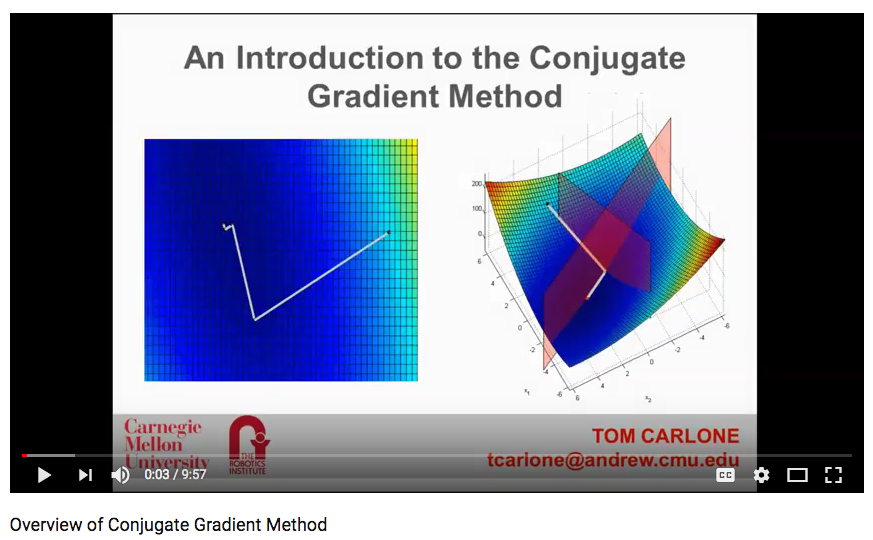
\includegraphics[width=.8\textwidth]{youtubeCG}
\end{center}


\end{frame}




\begin{frame}[allowframebreaks]
	\frametitle{References}
\bibliographystyle{abbrv}
\bibliography{NumDNN}

\end{frame}
\end{document}
